
\documentclass[11pt,a4paper]{article}

\usepackage[margin=2cm,headheight=14pt]{geometry}
\usepackage[T1]{fontenc}
\usepackage[utf8]{inputenc}
\usepackage{lmodern}
\usepackage{microtype}
\usepackage{graphicx}
\usepackage{float}
\usepackage{booktabs}
\usepackage{xcolor}
\usepackage{listings}
\usepackage{hyperref}
\usepackage{fancyhdr}
\usepackage{enumitem}
\usepackage{tikz}
\usetikzlibrary{arrows.meta,positioning}

\definecolor{navy}{RGB}{22,65,110}
\definecolor{codebg}{RGB}{247,248,250}
\hypersetup{
  colorlinks=true,
  linkcolor=navy,
  urlcolor=navy,
  pdftitle={Cloud Computing Lab 4 -- Student Course Registration System},
  pdfauthor={Abdelhady Mohamed, Yousef Allam, Abdulrahman Magdy}
}
\pagestyle{fancy}
\fancyhf{}
\lhead{\small Cloud Computing -- Lab 4}
\rhead{\small Student Course Registration System}
\cfoot{\thepage}
\lstset{
  basicstyle=\ttfamily\small,
  backgroundcolor=\color{codebg},
  frame=single,
  breaklines=true,
  columns=fullflexible,
  showstringspaces=false,
  aboveskip=5pt,
  belowskip=7pt
}
\graphicspath{{images/}{../images/}{./}}

% Add the real university logo beside this .tex file, or in images/.
% The conditional avoids a compile failure if the logo has not yet been copied.
\newcommand{\universitylogo}{%
  \IfFileExists{Logo_ZC_2.png}{
\includegraphics[width=7cm]{Logo_ZC_2.png}}{%
    \IfFileExists{images/Logo_ZC_2.png}{
\includegraphics[width=7cm]{images/Logo_ZC_2.png}}{%
      \IfFileExists{../images/Logo_ZC_2.png}{
\includegraphics[width=7cm]{../images/Logo_ZC_2.png}}{%
        \fbox{\parbox[c][1.2cm][c]{3.3cm}{\centering\small Add\\Logo\_ZC\_2.png}}%
      }%
    }%
  }%
}
\newcommand{\screensingle}[2]{%
\begin{figure}[H]\centering
  \IfFileExists{images/#1}{\includegraphics[width=0.9\linewidth,height=0.32\textheight,keepaspectratio]{images/#1}}{%
  \IfFileExists{../images/#1}{\includegraphics[width=0.9\linewidth,height=0.32\textheight,keepaspectratio]{../images/#1}}{%
  \IfFileExists{#1}{\includegraphics[width=0.9\linewidth,height=0.32\textheight,keepaspectratio]{#1}}{%
  \fbox{\parbox[c][2cm][c]{0.85\linewidth}{\centering Missing screenshot: \texttt{#1}}}}}}
  \caption{#2}
\end{figure}
}
\newcommand{\screenpair}[4]{%
\begin{figure}[H]\centering
  \begin{minipage}{0.485\linewidth}\centering
  \IfFileExists{images/#1}{\includegraphics[width=\linewidth,height=0.24\textheight,keepaspectratio]{images/#1}}{%
  \IfFileExists{../images/#1}{\includegraphics[width=\linewidth,height=0.24\textheight,keepaspectratio]{../images/#1}}{%
  \IfFileExists{#1}{\includegraphics[width=\linewidth,height=0.24\textheight,keepaspectratio]{#1}}{%
  \fbox{\parbox[c][1.8cm][c]{0.9\linewidth}{\centering Missing: \texttt{#1}}}}}}
  \caption{#2}
  \end{minipage}\hfill
  \begin{minipage}{0.485\linewidth}\centering
  \IfFileExists{images/#3}{\includegraphics[width=\linewidth,height=0.24\textheight,keepaspectratio]{images/#3}}{%
  \IfFileExists{../images/#3}{\includegraphics[width=\linewidth,height=0.24\textheight,keepaspectratio]{../images/#3}}{%
  \IfFileExists{#3}{\includegraphics[width=\linewidth,height=0.24\textheight,keepaspectratio]{#3}}{%
  \fbox{\parbox[c][1.8cm][c]{0.9\linewidth}{\centering Missing: \texttt{#3}}}}}}
  \caption{#4}
  \end{minipage}
\end{figure}
}

\begin{document}

% ---------------- Cover ----------------
\begin{titlepage}
\centering
\vspace*{0.2cm}
\universitylogo

\vspace{0.5cm}
{\Large\textbf{University of Science and Technology at Zewail City}}\\[0.15cm]
{\large Communications and Information Engineering}\\[0.6cm]
{\large\textbf{Cloud Computing -- Lab 4 Assignment}}\\[0.8cm]
\rule{\linewidth}{1pt}\\[0.35cm]
{\huge\bfseries Student Course Registration System}\\[0.2cm]
{\Large Multi-Tier Deployment with Docker Compose}\\[0.35cm]
\rule{\linewidth}{1pt}\\[0.8cm]

\begin{tabular}{p{6cm}p{5cm}}
\toprule
\textbf{Team member} & \textbf{Student ID}\\
\midrule
Abdelhady Mohamed & 202201172\\
Yousef Allam & 202200286\\
Abdulrahman Magdy & 202200341\\
\bottomrule
\end{tabular}

\vspace{0.7cm}
\begin{tabular}{p{4.5cm}p{8cm}}
\textbf{Assigned host port} & 8072 ($8000+72$)\\
\textbf{Repository} & \url{https://github.com/3bdelhadYy/Multi-Tier-Application-with-Docker-Compose}\\
\textbf{Environment} & Ubuntu on WSL2 with Docker Compose\\
\end{tabular}

\vfill
{\small October 2026}
\end{titlepage}

\tableofcontents
\newpage

\section{Introduction and Objectives}
This lab deploys a Student Course Registration System using Docker Compose. The application lets users view courses, manage students, and register students in courses. The main goals are to run a three-tier application, separate services with Docker networks, publish only the assigned frontend port, preserve database records using a named volume, and demonstrate basic monitoring and recovery.

\section{System Architecture}
The system contains three services:
\begin{itemize}[leftmargin=*]
  \item \textbf{Frontend:} Nginx serves the HTML, CSS, and JavaScript interface and forwards \texttt{/api/} requests to the backend.
  \item \textbf{Backend:} FastAPI handles application requests and communicates with PostgreSQL.
  \item \textbf{Database:} PostgreSQL stores course, student, and registration records.
\end{itemize}

\begin{figure}[H]
\centering
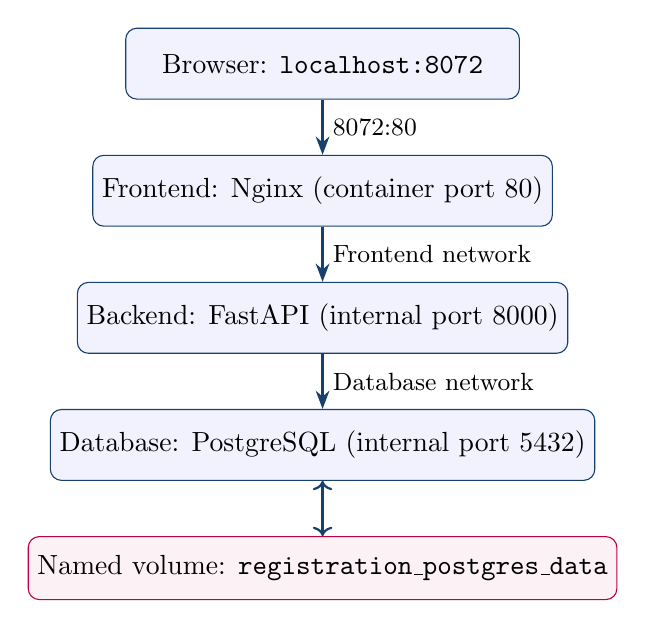
\begin{tikzpicture}[
  node distance=0.7cm,
  service/.style={draw=navy,rounded corners,fill=blue!5,align=center,minimum width=5cm,minimum height=0.9cm},
  arr/.style={-{Stealth},thick,draw=navy}
]
\node[service] (browser) {Browser: \texttt{localhost:8072}};
\node[service,below=of browser] (front) {Frontend: Nginx (container port 80)};
\node[service,below=of front] (back) {Backend: FastAPI (internal port 8000)};
\node[service,below=of back] (db) {Database: PostgreSQL (internal port 5432)};
\node[draw=purple,rounded corners,fill=purple!5,align=center,below=of db,minimum width=5cm,minimum height=0.8cm] (vol) {Named volume: \texttt{registration\_postgres\_data}};
\draw[arr] (browser) -- node[right,font=\small]{8072:80} (front);
\draw[arr] (front) -- node[right,font=\small]{Frontend network} (back);
\draw[arr] (back) -- node[right,font=\small]{Database network} (db);
\draw[arr,<->] (db) -- (vol);
\end{tikzpicture}
\caption{Three-tier application architecture and persistent database storage.}
\end{figure}

The frontend and backend share \texttt{registration\_frontend\_network}. The backend and database share \texttt{registration\_database\_network}. The frontend is not attached to the database network. Only the frontend publishes a host port; the backend and database are intended for internal communication.

\section{Deployment and Main Commands}
The services are defined in \texttt{compose.yaml}. Compose builds the frontend and backend images, starts PostgreSQL, checks database readiness, and connects the services to their required networks. The database uses a named volume so that its data is not stored only in the container's writable layer.

The following are the main commands used during setup and deployment:

\begin{lstlisting}
docker --version
docker compose version
docker run --rm hello-world
docker images
docker compose up -d --build
docker compose ps
\end{lstlisting}

Open the application at \url{http://localhost:8072}. The expected services are frontend, backend, and database. The database should become healthy before the backend relies on it.

\section{Networking and Port Configuration}
The project uses two bridge networks:
\begin{itemize}[leftmargin=*]
  \item \texttt{registration\_frontend\_network}: frontend and backend.
  \item \texttt{registration\_database\_network}: backend and database.
\end{itemize}
This segmentation limits direct connectivity: the frontend does not join the database network. The frontend is published as host port 8072 to container port 80. Backend port 8000 and PostgreSQL port 5432 are not published to the host.

\begin{lstlisting}
docker network inspect registration_frontend_network
docker network inspect registration_database_network
curl -i http://localhost:8072/api/health
\end{lstlisting}

\section{Database and Persistence}
The database stores records in the \texttt{students}, \texttt{courses}, and \texttt{registrations} tables. The application uses relational constraints to protect data integrity and prevents duplicate student-course registrations. Course capacity is checked by the backend when registrations are submitted.

The PostgreSQL data directory is backed by the named volume \texttt{registration\_postgres\_data}. To test persistence, the application data was queried before and after removing and recreating containers. The important safety note is to use \texttt{docker compose down}, not \texttt{docker compose down -v}, because \texttt{-v} removes named volumes.

\begin{lstlisting}
docker exec -it registration-db psql -U postgres_user -d course_registration_db -c "\dt"
docker compose down
docker compose up -d
\end{lstlisting}

\section{Testing, Troubleshooting, and Recovery}
The health endpoint \texttt{/api/health} is used to check application and database availability. To demonstrate troubleshooting, the database service can be stopped, backend logs inspected, and the database restarted. The exact response should be described according to the captured output.

\begin{lstlisting}
docker compose stop db
curl -i http://localhost:8072/api/health
docker compose logs --tail=50 backend
docker compose start db
docker compose ps
\end{lstlisting}

After restarting the database, check that it is healthy and retry the health endpoint. Logs help identify database connectivity problems. Do not remove the volume during this test.

\section{Screenshots and Results}
The following screenshots document the setup, application functionality, database, networks, persistence test, and troubleshooting. Captions describe the evidence; the images themselves should be checked against the actual observed outputs.

\subsection{Environment and Deployment}
\screenpair{01-docker-versions-hello-world.jpg}{Docker and Compose versions and the hello-world test.}{02-docker-images.jpg}{Available Docker images.}
\screenpair{03-project-tree.jpg}{Project directory structure.}{04-compose-ps.jpg}{Compose service status.}

\subsection{Application and Database}
\screenpair{05-application-courses.jpg}{Course management interface.}{06-application-students.jpg}{Student management interface.}
\screenpair{07-registration-and-course-roster.jpg}{Registration records and course roster.}{08-database-rows.jpg}{PostgreSQL table and registration inspection.}

\subsection{Network and Health Check}
\screenpair{09.1a-frontend-network.jpg}{Frontend network inspection.}{09.1b-database-network.jpg}{Database network inspection.}
\screenpair{09.2a-frontend-network.jpg}{Additional frontend network evidence.}{09.2b-database-network.jpg}{Additional database network evidence.}
\screensingle{10-port-and-health-check.jpg}{Port mapping and API health check.}

\subsection{Persistence and Recovery}
\screenpair{11-persistence-before.jpg}{Data before container recreation.}{12-persistence-after.jpg}{Data after container recreation.}
\screensingle{13-service-failure-and-logs.jpg}{Database failure, logs, and recovery evidence.}

\section{Conclusion}
The project demonstrates a three-tier application managed by Docker Compose. Nginx provides the single host entry point on port 8072, FastAPI handles application logic, and PostgreSQL stores relational data. Separate bridge networks limit direct connectivity between tiers, while a named volume supports data persistence across container recreation. The screenshots and commands provide evidence of deployment, application use, database inspection, and troubleshooting.

\end{document}
